%% ----------------------------------------------------------------
%% Thesis.tex -- MAIN FILE (the one that you compile with LaTeX)
%% ---------------------------------------------------------------- 

% Set up the document
\documentclass[a4paper, 11pt, oneside]{Thesis}  % Use the "Thesis" style, based on the ECS Thesis style by Steve Gunn

% Include any extra LaTeX packages required
\usepackage[square, numbers, comma, sort&compress]{natbib}  % Use the "Natbib" style for the references in the Bibliography
\usepackage[T1]{fontenc}
\usepackage{verbatim}  % Needed for the "comment" environment to make LaTeX comments
\usepackage{vector}  % Allows "\bvec{}" and "\buvec{}" for "blackboard" style bold vectors in maths
\usepackage{graphicx} % Allows for "\includegraphics{}" for images
\usepackage{float}
\graphicspath{ {Images/} } % Set location of images
\hypersetup{urlcolor=black, colorlinks=true}  % Colours hyperlinks in blue, but this can be distracting if there are many links.
\usepackage{listings}
\usepackage{upquote}
\usepackage{color}
\definecolor{bluekeywords}{rgb}{0.13,0.13,1}
\definecolor{greencomments}{rgb}{0,0.5,0}
\definecolor{redstrings}{rgb}{0.9,0,0}
\lstdefinelanguage{FSharp}%
{morekeywords={let, new, match, with, rec, open, module, namespace, type, of, member, % 
and, for, while, true, false, in, do, begin, end, fun, function, return, yield, try, %
mutable, if, then, else, cloud, async, static, use, abstract, interface, inherit, finally },
  otherkeywords={ let!, return!, do!, yield!, use! },
  keywordstyle=\color{bluekeywords},
  sensitive=true,
  basicstyle=\ttfamily\small,
	breaklines=true,
  xleftmargin=\parindent,
  aboveskip=\bigskipamount,
	tabsize=2,
  morecomment=[l][\color{greencomments}]{///},
  morecomment=[l][\color{greencomments}]{//},
  morecomment=[s][\color{greencomments}]{{(*}{*)}},
  morestring=[b]",
  showstringspaces=false,
  literate={`}{\`}1,
  stringstyle=\color{redstrings},
}
\lstset{language=FSharp}
%% ----------------------------------------------------------------
\begin{document}
\frontmatter      % Begin Roman style (i, ii, iii, iv...) page numbering

% Set up the Title Page
\title  {A Multi-Channel Data Transfer Protocol Using Asynchronous Technology}
\authors  {\texorpdfstring
            {William Czifro}
            {William Czifro}
            }
\addresses  {\groupname\\\deptname\\\univname}  % Do not change this here, instead these must be set in the "Thesis.cls" file, please look through it instead
\date       {\today}
\subject    {}
\keywords   {}

\maketitle
%% ----------------------------------------------------------------

\setstretch{1.3}  % It is better to have smaller font and larger line spacing than the other way round

% Define the page headers using the FancyHdr package and set up for one-sided printing
\fancyhead{}  % Clears all page headers and footers
\rhead{\thepage}  % Sets the right side header to show the page number
\lhead{}  % Clears the left side page header

\pagestyle{fancy}  % Finally, use the "fancy" page style to implement the FancyHdr headers

%% ----------------------------------------------------------------
% Declaration Page required for the Thesis, your institution may give you a different text to place here
% \Declaration{

% \addtocontents{toc}{\vspace{1em}}  % Add a gap in the Contents, for aesthetics

% I, AUTHOR NAME, declare that this thesis titled, `THESIS TITLE' and the work presented in it are my own. I confirm that:

% \begin{itemize} 
% \item[\tiny{$\blacksquare$}] This work was done wholly or mainly while in candidature for a research degree at this University.
 
% \item[\tiny{$\blacksquare$}] Where any part of this thesis has previously been submitted for a degree or any other qualification at this University or any other institution, this has been clearly stated.
 
% \item[\tiny{$\blacksquare$}] Where I have consulted the published work of others, this is always clearly attributed.
 
% \item[\tiny{$\blacksquare$}] Where I have quoted from the work of others, the source is always given. With the exception of such quotations, this thesis is entirely my own work.
 
% \item[\tiny{$\blacksquare$}] I have acknowledged all main sources of help.
 
% \item[\tiny{$\blacksquare$}] Where the thesis is based on work done by myself jointly with others, I have made clear exactly what was done by others and what I have contributed myself.
% \\
% \end{itemize}
 
 
% Signed:\\
% \rule[1em]{25em}{0.5pt}  % This prints a line for the signature
 
% Date:\\
% \rule[1em]{25em}{0.5pt}  % This prints a line to write the date
% }
% \clearpage  % Declaration ended, now start a new page

%% ----------------------------------------------------------------
% The "Funny Quote Page"
% \pagestyle{empty}  % No headers or footers for the following pages

% \null\vfill
% % Now comes the "Funny Quote", written in italics
% \textit{``Write a funny quote here.''}

% \begin{flushright}
% If the quote is taken from someone, their name goes here
% \end{flushright}

% \vfill\vfill\vfill\vfill\vfill\vfill\null
% \clearpage  % Funny Quote page ended, start a new page
%% ----------------------------------------------------------------

% The Abstract Page
% \addtotoc{Abstract}  % Add the "Abstract" page entry to the Contents
% \abstract{
% \addtocontents{toc}{\vspace{1em}}  % Add a gap in the Contents, for aesthetics

% The Thesis Abstract is written here (and usually kept to just this page). The page is kept centered vertically so can expand into the blank space above the title too\ldots

% }

% \clearpage  % Abstract ended, start a new page
%% ----------------------------------------------------------------

% \setstretch{1.3}  % Reset the line-spacing to 1.3 for body text (if it has changed)

% The Acknowledgements page, for thanking everyone
% \acknowledgements{
% \addtocontents{toc}{\vspace{1em}}  % Add a gap in the Contents, for aesthetics

% The acknowledgements and the people to thank go here, don't forget to include your project advisor\ldots

% }
% \clearpage  % End of the Acknowledgements
%% ----------------------------------------------------------------

\pagestyle{fancy}  %The page style headers have been "empty" all this time, now use the "fancy" headers as defined before to bring them back


%% ----------------------------------------------------------------
% \lhead{\emph{Contents}}  % Set the left side page header to "Contents"
\tableofcontents  % Write out the Table of Contents

%% ----------------------------------------------------------------
% \lhead{\emph{List of Figures}}  % Set the left side page header to "List if Figures"
\listoffigures  % Write out the List of Figures

%% ----------------------------------------------------------------
% \lhead{\emph{List of Tables}}  % Set the left side page header to "List of Tables"
\listoftables  % Write out the List of Tables

%% ----------------------------------------------------------------
% \lhead{\emph{List of Listings}}  % Set the left side page header to "List of Listings"
 \lstlistoflistings  % Write out the List of Listings

%% ----------------------------------------------------------------
\setstretch{1.5}  % Set the line spacing to 1.5, this makes the following tables easier to read
\clearpage  % Start a new page
% \lhead{\emph{Abbreviations}}  % Set the left side page header to "Abbreviations"
\listofsymbols{ll}  % Include a list of Abbreviations (a table of two columns)
{
% \textbf{Acronym} & \textbf{W}hat (it) \textbf{S}tands \textbf{F}or \\
\textbf{FTP}   & \textbf{F}ile \textbf{T}ransfer \textbf{P}rotocol \\
\textbf{MCDTP} & \textbf{M}ulti-\textbf{C}hannel \textbf{D}ata \textbf{T}ransfer \textbf{P}rotocol \\
\textbf{NCP}   & \textbf{N}etwork \textbf{C}ontrol \textbf{P}rogram \\
\textbf{RFC}   & \textbf{R}equest \textbf{F}or \textbf{C}omment \\
\textbf{RTT}   & \textbf{R}ound \textbf{T}rip \textbf{T}ime \\
\textbf{TCP}   & \textbf{T}ransmission \textbf{C}ontrol \textbf{P}rotocol \\
\textbf{UDP}   & \textbf{U}ser \textbf{D}atagram \textbf{P}rotocol \\

}

%% ----------------------------------------------------------------
% \clearpage  % Start a new page
% \lhead{\emph{Physical Constants}}  % Set the left side page header to "Physical Constants"
% \listofconstants{lrcl}  % Include a list of Physical Constants (a four column table)
% {
% % Constant Name & Symbol & = & Constant Value (with units) \\
% Speed of Light & $c$ & $=$ & $2.997\ 924\ 58\times10^{8}\ \mbox{ms}^{-\mbox{s}}$ (exact)\\

% }

%% ----------------------------------------------------------------
% \clearpage  %Start a new page
% \lhead{\emph{Symbols}}  % Set the left side page header to "Symbols"
% \listofnomenclature{lll}  % Include a list of Symbols (a three column table)
% {
% % symbol & name & unit \\
% $a$ & distance & m \\
% $P$ & power & W (Js$^{-1}$) \\
% & & \\ % Gap to separate the Roman symbols from the Greek
% $\omega$ & angular frequency & rads$^{-1}$ \\
% }
%% ----------------------------------------------------------------
% End of the pre-able, contents and lists of things
% Begin the Dedication page

% \setstretch{1.3}  % Return the line spacing back to 1.3

% \pagestyle{empty}  % Page style needs to be empty for this page
% \dedicatory{For/Dedicated to/To my\ldots}

% \addtocontents{toc}{\vspace{2em}}  % Add a gap in the Contents, for aesthetics


%% ----------------------------------------------------------------
\mainmatter	  % Begin normal, numeric (1,2,3...) page numbering
\pagestyle{fancy}  % Return the page headers back to the "fancy" style

% Include the chapters of the thesis, as separate files
% Just uncomment the lines as you write the chapters

\chapter{Introduction}

Computer networking has a firm presence in many modern applications. Applications for social media, video streaming, and many other types of content rely on computer networking to serve content to the users of these types of applications. Whether the communication be via a server using the Hypertext Transfer Protocol (HTTP) or a server using the WebSocket Protocol (WebSockets), the common denominator is the Transmission Control Protocol (TCP) \cite{fielding1999hypertext}\cite{fette2011websocket}. As an underlying protocol to HTTP and WebSockets, TCP provides these higher level protocols, as well as other protocols that use TCP, reliability in communication and data integrity \cite{cerf1978specification}. These assurances offered by TCP have associated costs that directly impact transfer rate and network utilization, or bandwidth.

Many proposed methods for improving the transfer rate and network utilization include solutions like \cite{brakmo1995tcp}\cite{wei2006fast}\cite{xu2004binary}\cite{ha2008cubic} as well as others mentioned in \cite{ha2008cubic}\cite{He2002}. These solutions tend to focus on fine tuning TCP to use a large sliding window or change how the congestion control mechanism of TCP handles a packet loss event. As physical connections increase in bandwidth, fine tuning TCP may not be enough to improve performance, especially for connections that have large Round-Trip-Times (RTT) and/or under utilize bandwidth \cite{Fan2010} on network links like \cite{Pfister2001} and other Gigabit links.

A different approach has been to focus on creating new higher level protocols, or Application layer protocols. Works like \cite{Allman1995}\cite{Allman1997}\cite{Sivakumar2000psockets} used multiple TCP connections in parallel to try and improve performance without sacrificing reliability in communication. Parallelization poses two major challenges. The first is the additional work the application needs to do to handle multithreading in a way that addresses race conditions, deadlocks, and synchronicity. The second challenge is directly related to the degree of parallelism of a machine. For instance, if a machine has four hyperthreaded cores, it can support eight threads in parallel. In order to fully utilize the CPU, the application has to ensure that all eight threads are busy with work. If a thread goes idle, the application is not using the CPU to its fullest potential. Solutions that use parallelization may be able to improve bandwidth usage and transfer rate, but the shortcoming is under utilization of hardware rendering these solutions suboptimal.

Along with the use of parallel computing, there have been adaptations of the higher-level protocols and systems mentioned in \cite{Fan2010} that utilize UDP as the transport for packets from sender to receiver \cite{He2002}\cite{Fan2010}\cite{Aspera2016}\cite{Meiss2007}\cite{gu2007udt}. Using a UDP transport can be a viable method to mitigating under utilized networks. The reason for this is, unlike TCP, UDP does not employ any type of congrestion control or packet recovery \cite{postel1980user}. However, this means that in scenarios where the network is already congested, packets may be lost because UDP will attempt to send packets with no regard for the network conditions. Solutions like these that are UDP-based have to tackles the issue of communication reliability themselves. With increasing capabilities of physical connections with respect to bandwidth, a new challenge presents itself.

Aspera has noted that the challenge with Computer Networking is not so much with slow physical connections, but is instead with the end systems not being fast enough for the connection \cite{Fan2010}\cite{Aspera2016}. The path Aspera took involved building a custom end system that could operate faster to handle faster connections. The decision Aspera made begs the question, is it possible to achieve a faster end system by using a more generic technology?

This paper reviews an experimental protocol called Multi-Channel Data Transfer Protocol (MCDTP). The experimental protocol seeks address the aforementioned question by using asynchrony. This report discusses the design of the protocol, the architecture of the implementation, the performances of MCDTP, and the challenges faced by this project. The goal of this project is to illustrate the effects of asynchrony with respect to data processing in the context of Computer Networking.
 % Introduction

\chapter{Background}

In order to approach the problem in a unique way, it was necessary to have a background to the general problem and technologies used by other works as well as technologies used in this project.

\section{Networking}

TCP was invented in 1978 to provide a "reliable host-to-host" protocol for network communication \cite{cerf1978specification}. By using packet reception acknowledgements and congestion control, TCP gave reliability insurance over the Internet Protocol and became the standard for network communication in 1983 \cite{andrews2013who}. UDP was created in 1980 as an alternative to TCP \cite{postel1980user}\cite{kozierokr2005udp}. UDP was designed for applications that needed faster communication. TCP and UDP are now standard protocols in the Transport layer of the network stack.

\subsection{Optimizing TCP}

After the standardization of TCP and growing use of it as a transport protocol, optimizing TCP to transmit data faster has been the goal in these works \cite{brakmo1995tcp}\cite{wei2006fast}\cite{ha2008cubic}. 

TCP-Vegas \cite{brakmo1995tcp} uses the RTT to measure throughput and a lower bound threshold and upper bound threshold to perform congestion control. If the lower bound is greater than the measured throughput, TCP-Vegas will increase the sending rate of the packets. If the measured throughput exceeds the upper bound threshold, it throttles how fast the packets are being sent. Consequently, this method reduces the number of retransmits and the sliding window of TCP can continually move forward.

FAST \cite{wei2006fast} uses RTT and packet loss as measures for congestion control. This method tries to maximize bandwidth usage by being agressive with increasing window sizes until the RTT gets close to a threshold. FAST takes an optimistic approach when exceeding the threshold. It will slowly decrease the window size in hopes that the RTT had degraded for a brief moment. Only when it worsens does FAST aggressively decrease window size. As a result, all paths in a connection equally share the effects of a bottleneck and thus mitigating the ebbs and flows of traffic providing a consistent throughput.

CUBIC \cite{ha2008cubic} is the successor to the BIC-TCP congestion control system. This method treats window growth as a cubic function, using the concave profile on a loss event to increase back to the last recorded max window size, and the convex profile for exceeding the last recorded max window size. This approach allows for the window size to be consistently near the recorded max window size. Due to this, there is a high utilization of the network.

\subsection{Application Layer Protocols}

The Transport layer protocols like TCP and UDP are the foundation for higher level protocols that attempt to optimize throughput at the Application layer, \cite{Fan2010}\cite{Allman1997}\cite{Allman1995}\cite{Aspera2016}\cite{Meiss2007}\cite{gu2007udt}\cite{lai2009designing}\cite{He2002}\cite{Sivakumar2000psockets}.

\subsubsection{UDP Based Protocols}

Tsunami \cite{Meiss2007} uses both UDP and TCP to transmit data. Tsunami uses UDP for sending the payload and TCP as a feedback loop. The TCP connection provides signaling for packet loss, ratransmission requests, error reporting, and completion report. For retransmission, the server will interrupt the flow to resend the data block in which the packet loss occurred. This approach achieved a 400-450 Mbps throughput when transferring a 5 GB file.

RBUDP \cite{He2002} is similar to Tsunami in its mechanics. RBUDP uses a TCP connection to send messages between sender and receiver. The major difference is the retransmit part. RBUDP retransmits packets over UDP after the "bulk data transmission phase" has finished, which is repeated until all packets have made it to the receiver. RBUDP was able to upper bounded packet loss to 7\% and achieve a throughput of 550Mbps.

UDT \cite{gu2007udt} is strictly a UDP-based protocol that imposes a congestion control mechanism on top of that. Used to UDP sockets, one socket labeled "Sender", the other labeled "Receiver". The receiver socket would not only receiver data, but it would be used for sending control information. UDT used TCP like messages for congestion control and reliability insurance. During a transfer from Chicago to Amsterdam, UDT had a throughput of 940Mbps over a 1Gbps link.

Aspera's fasp protocol \cite{Aspera2016}\cite{Fan2010} is a UDP-based protocol that uses a rate-based control system by using early congestion notification and random early detection to adjust the rate of the transmission. fasp handles ratransmissions by resending packets at a rate that makes use of available bandwidth. This provides a continuous flow of data. Network utilization is kept at near 100\%.

\subsubsection{Network Stack Optimization}

ADTS \cite{lai2009designing} is a replacement layer for the Network and Transport layer and is intended to be used of InfiniBand \cite{Pfister2001} (InfiniBand is network stack that treats network traffic as communication rather than bussed data). ADTS uses a zero-copy communication system that reduces latency on the host. It mitigates the need for the CPU to copy data to different places in memory according to the application's needs. Instead, a send will send data directly to an address in memory. This mitigation of unnecessary CPU usage and allowance of direct memory access provided a data transfer speed increase of 65\%.

\subsubsection{Optimization Through Concurrency}

XFTP \cite{Allman1995}\cite{Allman1997} is a modified version of FTP \cite{postel1980user} that uses multiple TCP connections to transfer a single file. The file is divided into records, with the condition that the number of records is greater than the number of connections. When a connection has the resources to send, it is assigned a record to transmit. The receiver reconstructs the original file by placing records in their correct positions. XFTP could achieve a 90\% network utilization using 8 connections.

PSockets \cite{Sivakumar2000psockets} is socket programming library that enables the use of parallel TCP sockets. The library provides simple send and receive functions that abstract the mechanics of PSocket. The passed in data is segmented and sent across multiple TCP connections. The receiver reassembles the received data back into its original form. PSockets manages multiple sockets asynchronously so that sockets do not need to simultaneously share resources. 


\section{Asynchrony}

Though this paper does not focus on asynchrony, it is a part of the design choices and implementation of this project and thus is worth reviewing. Asynchrony started out as a way for processes to communicate with each other using unbounded buffer channels \cite{Josephs1989}. A process uses in and out channels for messaging and sharing data with other processes. The purpose is to provide non-blocking behavior. A process does not need to wait for a message or a piece of data to continue doing work, it reacts to incoming messages. This concept has worked its way into programming models and work scheduling \cite{Guo2009}\cite{Leijen2009}\cite{syme2011f}

\subsection{Scheduling Asynchronous Work}

There are two major policies for scheduling asynchronous work, work-first and help-first \cite{Guo2009}. The work-first policy, also known as work-stealing, schedules spawned tasks for immediate execution and any continuation of that task is placed in a queue where other workers can steal from. This policy is particularly useful in situations where workers a busy an rarely need to steal from other workers. The help-first policy takes the opposite approach. A worker will ask help from other workers to begin executing spawned tasks. The continuations of the task are executed by the original worker. This policy is useful when stealing is very frequent because stealing can be implemented in parallel and thus increases the throughput of scheduled tasks.

\subsection{Asynchronous Programming Models}

Implementing asynchrony into a language or project can be very challenging. The theory of asynchrony suggests that communication channels need to be unbounded \cite{He1990}. This is not feasible. This paper and project focus on newer technologies, but for the sake of posterity it is with mentioning former projects like Cilk and JSD that paved the way for implementing asynchrony \cite{sutcliffe1988jackson}\cite{Cameron1986}\cite{Frigo1998}.

\subsubsection{.NET Framework Implementation}

The .NET Framework by Microsoft provides implementations of asynchrony in their languages C\# and F\# \cite{syme2011f}\cite{Leijen2009}. The C\# language received an update in 2009 that add the TPL library that provides asynchronous capabilities in C\#. In later updates, C\# was introduced with the keywords "async" and "await" that allowed for simpler asynchronous programming \cite{alexdavies2012}. This update meant any synchronous method could be transformed into an asynchronous method by adding only these keywords because the compiler transforms the user code into truly asynchronous code. The asynchronous feature of F\# uses the "async" keyword as well, however, the F\# compiler provides more granularity in turning a block of user code into asynchronous code \cite{syme2011f}. Both languages use the TPL library \cite{Leijen2009}\cite{msftVFS}.
 % Related Work

\chapter{Design}

The architectural design of MCDTP uses both TCP and UDP connections. Like the works \cite{He2002,Fan2010,Aspera2016,Meiss2007}, MCDTP uses the UDP transport protocol for the data transfer and the TCP socket is used for exchanging messages between the server and client. The experimental component of this protocol is the lack of congestion control. As mentioned in \cite{Fan2010} and \cite{Aspera2016}, the observed bottleneck resides on the hosts of an end-to-end transfer. MCDTP seeks to mitigate this through multiple asynchronous data channels where the number of channels is determined when implementing this protocol. A channel acts as a pipe from disk to socket and vice versa. This is how MCDTP tries to provide a continuous data flow. Implementation details are further discussed in Chapter \ref{chp:impl}. As a disclaimer, the term ``packet(s)'' hereinafter does not refer to Transport or Network layer packets, the term is used to refer to an Application layer structure used by MCDTP.

\section{Protocol Design}\label{sec:proto-des}

The MCDTP protocol focuses on being minimalistic and lean to try and minimize the needed time to process incoming messages or data. The protocol consists of three phases: a two step handshake phase, data transmission phase, and packet retransmission phase. For the sake of consistency and a lean design, control messages transmitted over the TCP connection are fixed to 15 bytes in length. Each packet is a header with an optional payload. All headers begin with two fields, ``ptype'' and ``subtype''. These two fields specify how the packet should be processed.

The UDP packet does not have a fixed size like the TCP packets. The size of the UDP packet is at minimum 13 bytes to accommodate for header fields and at maximum 64 kilobytes due to a limitation of the underlying Internet Protocol \cite{postel1981ip}. Unlike the TCP packets, UDP packets include payload size with packet size. Since UDP has the option of a payload, when one exists, a second read from the stream will be required to grab the payload. With the TCP packet, it is guaranteed that a packet will be a set size and thus eliminates the need for a second read.

\subsection{Two Step Handshake}

As with many protocols, MCDTP has a handshake step for exchanging host specifications as well as information regarding the data that will be transferred. However, for the sake of extensibility, this handshake step is split into two distinct handshakes. This allows for expansions to MCDTP to include more features, i.e. file selection.

\subsubsection{Specification Handshake}

The specification handshake occurs when a client connects to the server. Figure \ref{fig:specs} illustrates the type of communication that happens during the handshake.

\begin{figure}[ht]
\centering
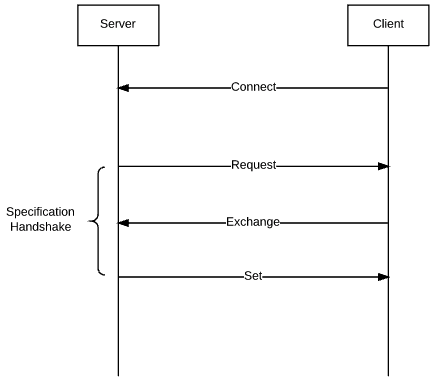
\includegraphics[scale=0.7]{SpecificationHandshake}
\caption{Illustration of Specification Handshake. This handshake is ensure that both client and server use the same specifications for a data transfer.}
\label{fig:specs}
\end{figure}

The packet structures in Figure \ref{fig:specs-struct} correspond to the handshake exchanges in Figure \ref{fig:specs}. The $Request$ message is how the server signals to the client that the server needs to know the specifications of the client. The specifications shared by the client are the ports of the open channels on the client. The client sends this data to the server using the $Exchange$ packet as a header that informs the server of how many port values are being sent. The server uses this exchanged specification to decide how many channels will be used and which ports the client should listen on. When deciding the number of channels, the server will side with the host that supports fewer channels. Once the server decides the specifications the client should use, the server responds with a $Set$ packet followed by the port values the client should use. The client will configure itself to use the channels corresponding to the received ports.

The $Exchange$ and $Set$ packet only express the number of port values that are being sent. The suggested implementation for receiving the port values is to represent port values as 32 bit integers, or 4 bytes, and leverage that fact while reading each port off of the stream. A more optimal approach is to calculate the payload size using the value from the packet header and the size of a port to read in all ports at once.

\begin{figure}[ht]
\centering
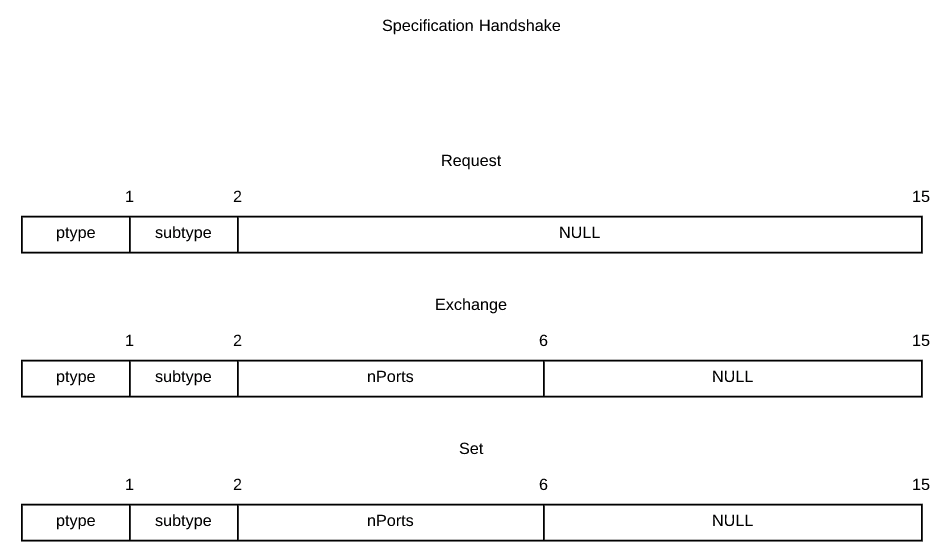
\includegraphics[scale=0.4]{SpecificationHandshakePacketStructures}
\caption{Packet Structure of Specification Handshake. The fields $ptype$ and $subtype$ are for identifying packets. The values of these fields are an implementation detail.}
\label{fig:specs-struct}
\end{figure}

\subsubsection{FTP Handshake}\label{subsec:ftp-hs}

Prior to transferring a file, MCDTP performs another handshake that is similar in design to the specification handshake, as can be seen in Figure \ref{fig:ftp-hs}.

\begin{figure}[ht]
\centering
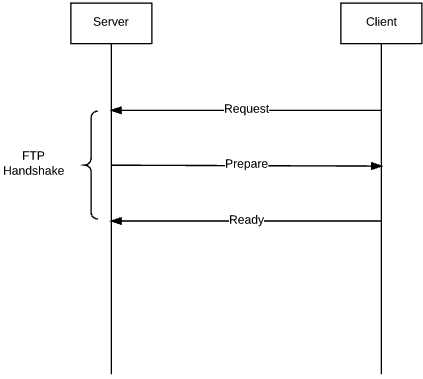
\includegraphics[scale=0.7]{FTPHandshake}
\caption{Illustration of FTP Handshake}
\label{fig:ftp-hs}
\end{figure}

This handshake acts as a concrete step before the data transmission phase and is minimal in design and purpose. This step is so that any asynchronous work that needs to be done first can finish as well as ensure both client and server are prepared for the data transmission phase, which is more of an implementation discussion and will be further discussed in Chapter \ref{chp:impl}. Figure \ref{fig:ftp-struct} is an illustration of the structure of each message in the handshake.

\begin{figure}[ht]
\centering
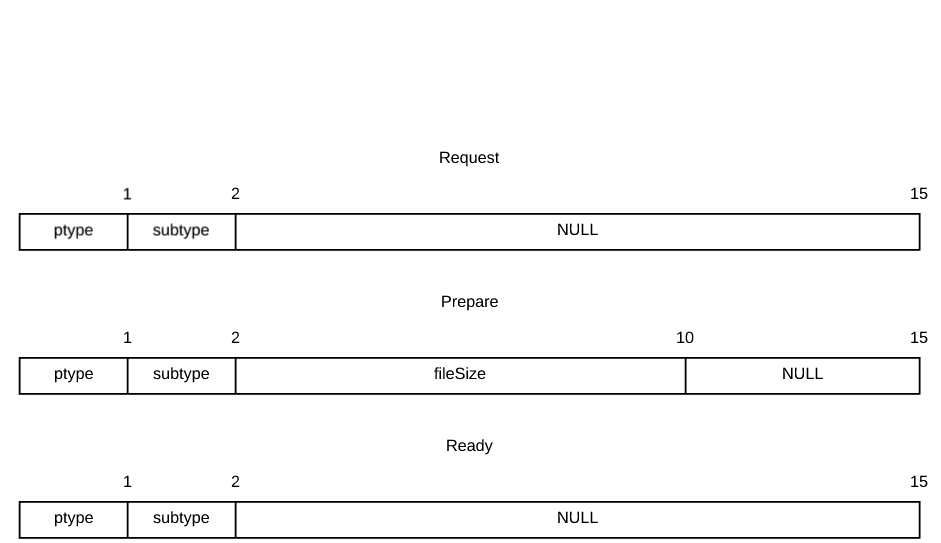
\includegraphics[scale=0.4]{FTPHandshakePacketStructures}
\caption{Packet Structure of FTP Handshake. The fields $ptype$ and $subtype$ are for identifying packets. The values of these fields are an implementation detail.}
\label{fig:ftp-struct}
\end{figure}

 The only information exchanged in this handshake is the size of the file that will be transferred, from server to client. Note that handling file selection has been omitted and will be further discussed in Chapter \ref{chp:c-fw}. Once the client is prepared for transfer and has signaled the server that it is ready, both hosts begin the data transmission phase of the MCDTP protocol.

\subsection{Data Transmission}

The data transmission phase is the second phase in the MCDTP protocol and is comprised mostly of the transmission of a file using the data channels setup in phase 1. The upper portion of Figure \ref{fig:data-tr} illustrates the communication between server and client. The packet retransmission phase and this phase have slight overlap, which is further discussed in Section \ref{subsec:pack-retr}.

\begin{figure}[ht]
\centering
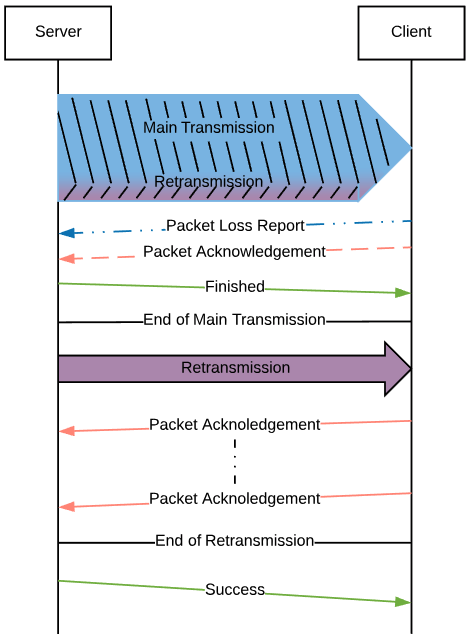
\includegraphics[scale=0.5]{DataTransfer}
\caption{Illustration of Data Transfer\\
The large arrow from server to client at the top represents the data flow for a single channel. The blue in this representation symbolizes the transmission of the file \cite{Meiss2007,He2002,gu2007udt,Fan2010,Aspera2016}.}
\label{fig:data-tr}
\end{figure}

The packet structure of the data transmitted over each channel is shown in Figure \ref{fig:data-tr-struct}. Note that the packet size is not definitively set. As stated previously, the packet size can range from $13B \leq size \leq 64KB$ and is something that needs to be set at an implementation level. The packet header fields ``seqNum'' and ``dLen'' are information regarding the payload of the UDP packet. The ``seqNum'' field is the position in file that the data should be written to. For the sake of being lean, the ``dLen'' field can be used to determine how much of the received payload is file data. This enables the implementation to read in a fixed amount of data. The ``flag'' field acts as a control flag. When the control flag is 0, the packet is a regular packet. A retransmitted packet has a flag value of 1 and 2 is to signal to the client that the channel is switching to the packet retransmission phase. The final packet is illustrated by the green communication line labeled ``Finished'' in Figure \ref{fig:data-tr}, which is sent over the UDP channel.

\begin{figure}[ht]
\centering
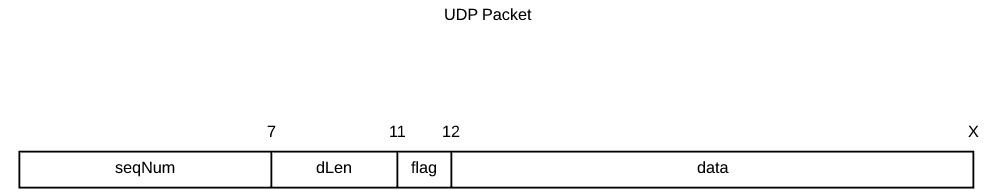
\includegraphics[scale=0.4]{DataTransferPacketStructure}
\caption{Packet Structure of Data Transfer (UDP Packet). The packet is variable in size.}
\label{fig:data-tr-struct}
\end{figure}

As previously mentioned, MCDTP is an experimental protocol. The experimental component attempts to perform a file transfer without the use of congestion control. The protocol tries to exploit the common operating system behavior that when a socket is created, it is given its own receive buffer. With each channel getting its own receive buffer, there is more space to hold incoming packets giving opportunity for handling more data at the Application layer.

\subsection{Packet Retransmission}\label{subsec:pack-retr}

The packet retransmission phase is capable of starting during the data transmission phase. The purpose of this is to recover packets along the way to minimize the duration of this phase and ultimately achieve a successful transfer faster. As can be seen in Figure \ref{fig:data-tr}, retransmission consumes a small portion of bandwidth so as not to impede upon the main transmission during the data transmission phase. The dashed communication lines labeled ``Packet Loss Report'' and ``Packet Acknowledgement'', which share the same structure as is evident in Figure \ref{fig:pack-rec-struct}, only occur when packet loss or packet recovery is detected and are sent over the TCP socket. The values for ``ptype'' and ``subtype'' are as follows:  Packet Loss Report) ``ptype'' = `t', ``subtype'' = `l' and Packet Acknowledgement) ``ptype'' = `t', ``subtype'' = `a'. Since the number of data channels is determined by the implementation, MCDTP uses the ``seqNum'' field to identify the UDP packet the message is in regards to and the ``port'' field to identify which channel the UDP packet was transferred over.

\begin{figure}[ht]
\centering
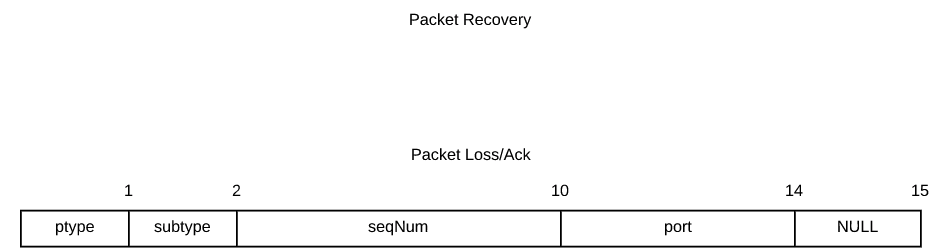
\includegraphics[scale=0.4]{PacketRecoveryStructure}
\caption{Packet Loss and Ack Report Structure for Packet Recovery}
\label{fig:pack-rec-struct}
\end{figure}

After the data transmission phase finishes, the packet retransmission phase is able to consume more bandwidth. The server will send a ``Finished'' packet to signal the client that the data channel on the server has transitioned to the retransmission phase, as illustrated in Figure \ref{fig:data-tr}. As previously mentioned, the control flag in the UDP packet has the value 2. This packet is placed at the head of the retransmission queue in order and is retransmitted until the client acknowledges the packet. This ensures that the server and client are both in the retransmission phase.

\begin{figure}[ht]
\centering
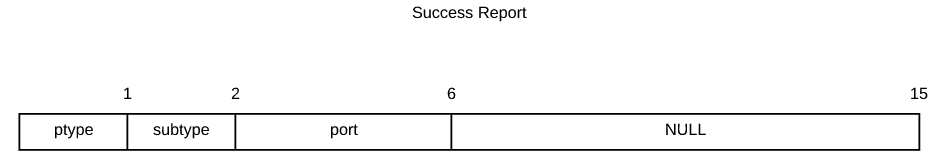
\includegraphics[scale=0.4]{SuccessPacketStructure}
\caption{Packet Structure of Success Report}
\label{fig:success-struct}
\end{figure}

Like RBUDP \cite{He2002}, a channel will continue this phase until the server has received an acknowledgement for all packets that are in recovery for that channel. Once all packets have been received, the server sends a success report, Figure \ref{fig:success-struct}, over TCP thus concluding the work the channel specified by the ``port'' field. The ``ptype'' and ``subtype'' in the success report are set to `t' and `S', respectively. Once all channels have succeeded, the session between the client and server is concluded. % Design

\chapter{Implementation}\label{chp:impl}

There are several paradigms used to construct the implementation of MCDTP. The construction of the implementation uses a hybrid of Functional Programming and Object-Oriented Programming to provide a modular architecture as well as making the project reactive to I/O events. As a side effect to using the paradigms, the programming API is very simple to use in other applications and/or wrappers.

\section{Why F\#?}

F\# was the chosen language for this project for a couple of reasons. The initial reason is the .NET Framework. As discussed in \cite{Leijen2009} and \cite{syme2011f}, the .NET Framework has a very robust built-in library that provides support for asynchronous tasking, especially for C\# and F\#. What makes this feature unprecedented, especially in C\# and F\#, is the embedded domain specific language (EDSL), often referred to as ``syntactic sugar", that the compiler uses to generate asynchronous code. The EDSL in F\#, referred to as ``computation expression" or ``workflow" in the F\# community, is especially powerful at composing asynchronous tasks.

Consider the following synchronous code:

\begin{lstlisting}[caption=Synchronous F\# Example]
let child() =
  System.Threading.Thread.Sleep(1000)
  printfn "Hello from child!"

let parent() =
  printfn "Parent calling child..."
  child()

parent()
\end{lstlisting}

The asynchronous equivalent is:

\begin{lstlisting}[caption=Asynchronous F\# Example,label={lst:async}]
let asyncChild =
  async {
    do! Async.Sleep(1000)
    printfn "Hello from child!"
  }

let asyncParent =
  async {
    printfn "Parent calling child..."
    do! asyncChild
  }

Async.RunSynchronously asyncParent
\end{lstlisting}

The transformation from synchronous code to asynchronous code is surprisingly simple thanks to the compiler, which is further discussed here \cite{syme2011f}. The ease of composing asynchronous tasks helps simplify constructing a reactive implementation, which is further discussed in section \ref{sec:reactive}.

The main reason for using F\# is the multi-paradigm aspect of the language \cite{Petricek}. F\# embodies Functional Programming---making it ideal for modular programming---as well as Object-Oriented Programming---which is great for reactive code---and Language Oriented Programming---enabling the creation of in-language DSLs to act as a declarative language for either configuring how something should behave, or providing a way to interact with an external resource or device without leaving F\#. This attribute has made F\# a prime candidate for constructing an implementation of MCDTP.

\section {Modular Architecture}

The modular approach to programming breaks a large codebase into smaller chunks called modules based on some criteria \cite{Microsystems2007}. Typically modules address a specific problem. Modules are also agnostic to outside code. This enables the ability to swap out modules for others. Since modules are identified partly by a version number, modules can be updated and not break projects using a module because they will be using a specific version of that module. These attributes of modular programming are the reason the implementation discussed in this paper of MCDTP was constructed with a modular architecture.

\begin{figure}[ht]
\centering
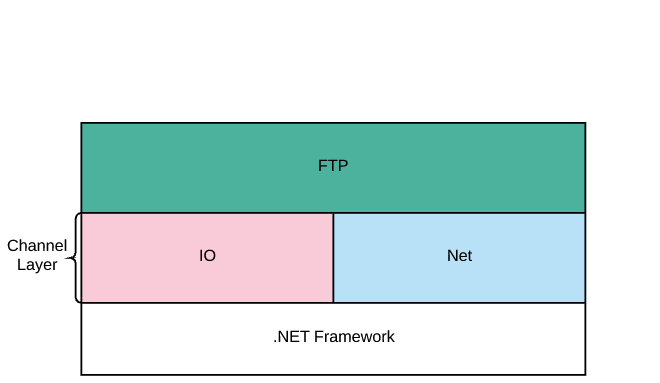
\includegraphics[scale=0.4]{MCDTPArchitecture}
\caption{MCDTP Modular Architecture}
\label{fig:mcdtp-arch}
\end{figure}

Figure \ref{fig:mcdtp-arch} illustrates the modular architecture of the MCDTP implementation, hereinafter referred to as MCDTPi. The top module is an FTP module (FTP) and depends on an I/O module (IO) and a Network module (Net). The .NET Framework is the base module of MCDTPi. This module is an external module that was not constructed while building MCDTPi; therefore, it will not be further discussed. Modules, and their respective submodules, will be reviewed in the order of dependency.

\subsection{Helper Modules}

There are two micro-modules that are used thoughout all modules and submodules in MCDTPi. The $Logging$ and $Utility$ modules, as seen in Figure \ref{fig:mcdtp-hm}, contain helper code that is commonly used throughout MCDTPi. The $Logging$ module was created to manage console and log file outputs for easier debugging. This module provides two configurable loggers, a console logger and a network logger. The console logger writes messages to a console. This logger is more of a general purpose logger. The network logger logs in app actions that relate to a socket I/O operation as well as packet loss. This logger writes to a file. Both loggers can be configured to log certain messages based on a priority level. $Logging$ provides a level for handling errors so that MCDTPi can be built more robust.

\begin{figure}[ht]
\centering
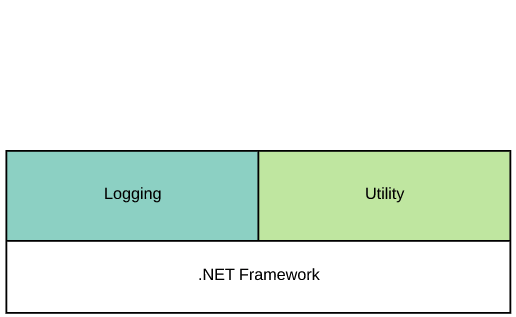
\includegraphics[scale=0.4]{MCDTPHelperModules}
\caption{MCDTP Helper Modules}
\label{fig:mcdtp-hm}
\end{figure}

The $Utility$ module provides code for type conversion, which is mostly used for serialization and deserialization purposes, as well as code for wrapping a function with a semaphor type data structure. This module is used mostly to provide abstractions to reocurring code snippets found throughout MCDTPi.

\subsection{IO Module}

The $IO$ module is one of the major modules to MCDTPi. The module handles all I/O related operations, except for socket I/O---see section \ref{sec:net} for more details. This module is composed of three submodules, as seen in Figure \ref{fig:mcdtp-io-arch}.

\begin{figure}[ht]
\centering
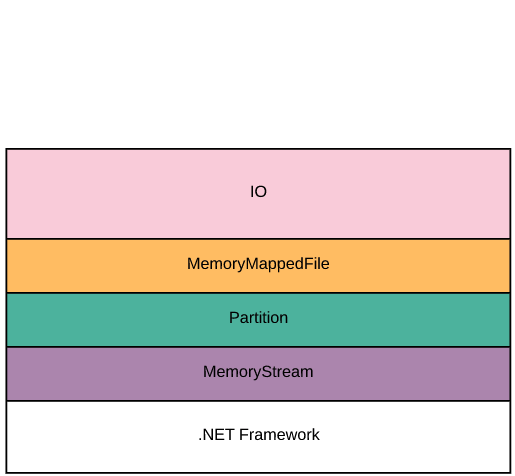
\includegraphics[scale=0.4]{MCDTPIOArchitecture}
\caption{MCDTP IO Architecture}
\label{fig:mcdtp-io-arch}
\end{figure}

\subsubsection{MemoryStream Sub-Module}

The $MemoryStream$ submodule is largely based on the $MemoryStream$ data structure found in the .NET Framework. The difference is that this submodule provides an unbounded buffer. The .NET Framework data structure has an upper bound on how much data can be written to the $MemoryStream$, which is $\frac{2^{32}}{2} - 1$---or the max value of a signed 32-bit integer. This would be a performance issue because it would restrict the amount of data that can be held in memory to 2GB. This is fine for low end machines, but many machines have 8GB or more of memory. The imposed upper bound needed to be mitigated through the use of a custom $MemoryStream$.

Instead of using a single byte array as the underlying container, MCDTPi uses a linked list of byte arrays to provide an unbounded container. Bytes are written to the end of the stream just like the original data structure; however, when a byte array fills up, an empty byte array is added to the end of the list so that more bytes can be added to the stream. As bytes are being read from a stream, the first array shrinks until it is empty, then it is removed from the list and the next byte array will be consumed. Though this stream is unbounded, its API uses bounded arrays as arguments and return values. The context in which this submodule will be used means that it should accept a bounded array as argument for writing to stream as well as returning a bounded array for read operations.

\subsubsection{Partition Sub-Module}

The $Partition$ submodule is actually a submodule to $MemoryMappedFile$ and uses $MemoryStream$ as a dependency. This submodule is used to read and write on part of a file. The ``part", or partition, has a $PartitionHandler$. This data structure is used to manager a file pointer within that part of the file. The $PartitionHandle$ keeps track of the state of the buffer and file pointer to ensure that any asynchronous I/O task, involving either the $MemoryStream$ or disk, do not overlap. This submodule is configurable with respect to how frequent a disk I/O operation should happen, whether it is read only or write only, and the console logger configuration it should use. Specifications like where the partition begins in the file and how large the partition is can be configured as well; however, it is highly recommended that those properties be set by the parent module $MemoryMappedFile$.

Additionally, $Partition$ handles special writes for data snippets in one of two ways. The initial method is to try and amend the buffer. The position in buffer is determined by the position in file the data snippet belongs to. The position in file is offset by the position of the beginning of the buffer. This gives how far into the buffer the snippet needs to be written. If the beginning of the buffer is positioned after the data snippet in file, then a write needs to happen that involves temporarily moving the file pointer to write the data snippet to disk and returning the file pointer back to its previous position.

\subsubsection{MemoryMappedFile Sub-Module}

The $MemoryMappedFile$ submodule is the top submodule in the $IO$ module. This submodule is the parent of $Partition$. It is inspired by the .NET Framework data structure of the same name. However, the difference lies in the functionality. Like the original data structure, $MemoryMappedFile$ is used to store large portions of a file in memory from different locations within the file. This submodule treats these portions as ``partitions", whereas the data structure treats them as ``views". A view in the data structure is a portion of a file that is loaded into memory. A partition is a portion of a file that has a dedicated file pointer and the partition is only partially loaded into memory---which would be the view of the partition.

Though it seems like a very insignificant difference, the major reason for creating this submodule was the ability to shift the view to a new position in file. The original data structure does not provide such functionality. Instead, to move a view would require creating a whole new view. This could lead to a struggle in managing memory. To prevent using too much memory, views would need to be smaller. Smaller views would mean more disk I/O operations to try and mitigate any interruption that may occur by either depleting the buffer representing the view, or filling buffer to capacity. This is why a custom submodule was constructed. To provide the ability to have a sliding view.

This functionality is offloaded to the child submodule $Partition$ since it is an action that happens to a partition of a file. $MemoryMappedFile$, instead, handles partitioning a file equally so that each partition is roughly of equal size. The configurable properties of a $MemoryMappedFile$ are the file name---used to identify a file to read or a new file to write to---the number of partitions to create---though it is recommended that $FTP$ set this---the $Partition$ configuration to use, and whether this file should be opened as read only or write only.

\subsection{Net Module}\label{sec:net}

Another core module to MCDTPi is the $Net$ module. This module handles network related actions, such as application level packet managing, parsing and composing raw data, and performing socket I/O operations. Like the $IO$ module, $Net$ is comprised of multiple submodules, as shown in Figure \ref{fig:mcdtp-net-arch}. Notice that the submodules are side-by-side instead of stacked like the $IO$ module. This means that the modules are independent of each other.

\begin{figure}[ht]
\centering
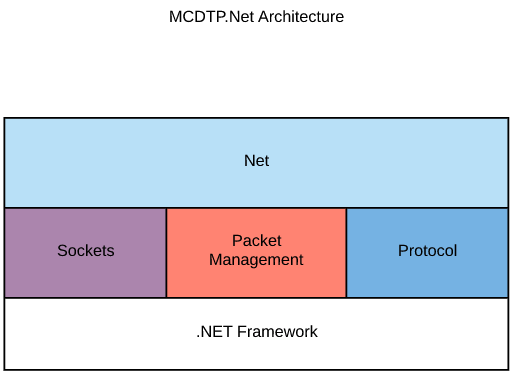
\includegraphics[scale=0.4]{MCDTPNetArchitecture}
\caption{MCDTP Net Architecture}
\label{fig:mcdtp-net-arch}
\end{figure}

\subsubsection{Protocol Sub-Module}

The Application Layer protocol that MCDTP defines is a very simplistic protocol. However, the implementation is a little more complex and thus, to help with maintainablility, MCDTPi has split the protocol into two modules and the $Protocol$ submodule is one of them. Divvying up the protocol like this means that any future work that changes the messages being sent and received only effects this submodule. This translates to faster compiling of code and in a production scenario means shorter down times. This submodule handles raw data that either came off the wire, or will be sent across the wire. $Protocol$ parses and composes raw data, or more commonly known as deserialize and serialize---sometimes called ``SerDe"---a data structure, respectively. Both of TCP and UDP packet structures discussed in section \ref{sec:proto-des} are handles by this submodule. $Protocol$ uses $Utility$ to convert raw bytes to more understandable primitive types. $Logging$ is also a dependency to provide output for error messaging so that when a message does not parse or compose correctly, the invalid input can be fetched for analysis if there is the need. The API of this submodule will be discussed in section \ref{sec:api}.

\subsubsection{Sockets Sub-Module}

All socket operations are housed in the $Sockets$ submodule. A configurable type class called $SocketHandle$ that wraps a socket is provided by this submodule. This type class is capable of performing pre- and post- socket I/O operations. This is more for compatability with $Protocol$. The pre- and post-operations are configurable so that any message handling service can be performed upon sending raw data or receiving raw data. Sending data is an asynchronous operation. Firstly, it is uses the provided asynchronous send function provided by .NET Framework. Secondly, it queues messages if an asynchronous operation is running. The receive operation is asynchronous as well thanks to the .NET Fremework, however, queueing receive requests is not supported. $SocketHandle$ is used for both TCP and UDP sockets and can be configured to use either protocol. IPv4 is the only supported version of the Internet Protocol at the moment. Section \ref{sec:api} will provide a code snippet on how the $Sockets$ module is used.

\subsubsection{PacketManagement Sub-Module}

The second submodule that implements the remainder of the UDP component of MCDTP is $PacketManagement$. This submodule is very complex. $PacketManagement$ is used to manage UDP packets. From the server's perspective, data is loaded from a source and converted to packets using $Protocol$. Packets are buffered and made accessible through a function call. When enough packets have been depleted, another batch is loaded. When there are no more packets to be loaded, the server buffers the final packet as per the design of MCDTP data transmission phase. The final packet is submitted to the front of the retransmit queue to ensure the client receives that packet.

When a packet is lost, the server gets a report that a packet, identified by a sequence number, has been lost. When $PacketManagement$ gets this report, the sequence number is submitted to a queue for processing, and, if the retransmit processor has not been initialized, it is setup to run on a configured interval. As reports come in, the retransmit processor will take a report and fetch the data from source and queue it up for retransmission. $PacketManagement$ is preconfigured to have 40 packets available for retransmission and send only 5 at a time, which is mostly to not obstruct the flow of the data transmission phase. The interval the retransmit processor executes is configurable. When the time is due to run the retansmit processor, it will copy up to 5 packets and push them on to the front of the main queue. During this time, the processor will also check to see if the retransmit queue needs to be reloaded. If so, any reports that are pending will be processed and moved to the retransmit queue. If there is no data to load and the rtransmit queue is empty, the retransmit processor will uninitialize itself, otherwise, it reinitializes itself for another interval. The acknowledgement system is fairly straight forward. Any acknowledged packets are removed from either queue.

On the client, packet loss is detected by gaps in the packet sequence numbers. Sequence numbers increase by the size of a packet. This is reliable because all packets are of the same size with the exception being the last packet. Thus, when a sequence number increases by more than the size of a packet, a packet is has been dropped. This detection occurs during the flush event. The flush event occurs when the buffer size exceeds a configured threshold. As a packet loss is detected, missing data is temporarily filled in with null values to ensure data remain in its correct position and a report list is compiled of all packets that have been lost. This list is sent over TCP to ensure the server knows which packets need to be retransmitted. When a packet is recovered, an acknowledgement is sent to the server. The data in the recovered packet gets submitted to $Partition$ for handling.

\subsection{FTP Module}

The $FTP$ module is the top module of MCDTPi. It interacts with the lower modules and helps $Net$ interact with $IO$, since they are side-by-side modules, by providing callback functions that can be used by either $Sockets$ or $PacketManagement$. $FTP$ manages data channels. It ensures that a data channel on the server matches a data channel on the client by pairing the start position of each partition to each port used by a UDP socket in ascending order--each channel is identified by the port. This is reliable because as per MCDTP design, ports are exchanged during the handshake. This module also handles all TCP communication and performs the associated action for a TCP packet. For instance, a packet loss report is directly handled by $FTP$ and forwards the report to the channel with the matching port identification. $FTP$ also prepares the $MemoryMappedFile$ submodule on both client and server. When both hosts are ready, $FTP$ initiates the transmission process. While this is running, $FTP$ exposes a state that represents the state of all channels. When all channels have succeeded, $FTP$ assumes the succeeded state. This module is configurable and propagates the configurations for the lower modules onward.

\section{Reactive}\label{sec:reactive}

Reactive Programming, also known as event-driven, is a paradigm that is used throughout MCDTPi. Reactive Programming seeks to make programs ``react" or respond to an event that has happened. As a result, there is never any code that is waiting for something to happen. Code only gets executed once an event has triggered it. The reason this is used is to more effectively use threads. Since code is never running waiting for something to happen, threads are not being wasted. With the exception of MCDTP.Net.Protocol and MCDTP.Utility, all modules and submodules are reactive.

When a UDP packet is received on the client, it gets processed by $Sockets$ and $Protocol$ and is submitted to $PacketManagement$. $PacketManagement$ decides if this packet will trigger a flush event or not. If it does not, the packet is simply added to the buffer. If it does, $PacketManagement$ asynchronously flushes the buffer by submitting the received data to $Partition$. If this action trigger a flush event within $Partition$, an internal asynchronous task will flush data to disk. This entire chain is reactive. Buffer flushing is an event, not something that is continuously running to see if data needs to be flushed.

The server follows a similar pattern. When a packet was successfully sent, an asynchronous event is triggered that queries a packet from $PacketManagement$. The query to $PacketManagement$ tries to pull a packet from buffer to send. This action can trigger an event within $PacketManagement$. If the buffer length falls below a threshold, a replenish event is triggered to pull data from $Partition$ and prepare packets from that data asynchronously. $Partition$ uses a similar event for the same task. When a packet is queried from $PacketManagement$, it is submitted to $Sockets$ and thus repeats the loop. This loop is asynchronous so any packets waiting to be sent will be processed in the meantime. Since this loop is reactive, $FTP$ jump starts the loop to get the process going.

\section{API}\label{sec:api}

F\# provides the ability to create computation expression like the $async$ keyword in listing \ref{lst:async}. MCDTPi takes advantage of this to provide a simple API for generating configurations used to configure the modules and submodules. The following code examples illustrate how simple it is to set up an MCDTPi instance on a server and client.

\begin{lstlisting}[caption=Server Example]
// create logger configurations
let console =
  loggerConfig {
    useConsole
    loggerId "Simple Console"
    logLevel LogLevel.Info
  }
let network =
  loggerConfig {
    networkOnly
    loggerId "Simple Network"
    logLevel LogLevel.Info
  }

// create socket configurations
let tcp = socketHandle { useTcp }
let udp = socketHandle { useUdp }

// create partition configuration
let partitionConfig =
  partition {
    // when buffer falls below 50MB, load another 50MB
    replenishThreshold (50 * 1000 * 1000)
    isReadOnly
    attachLogger console
  }

// create memoryMappedFile configuration
let mmfConfig =
  mmf {
    usePartitionConfig partitionConfig
    handleFile fileName
    isReadOnly
  }

// create ftp configuration
let ftpConfig =
  ftp {
    serverMode
    useConsole console
    monitorNetwork network
    configureUdp udp
    configureTcp tcp
    useParser Tcp.Parser.tryParse
    useComposer Tcp.Composer.tryCompose
    channelCount 4
  }

let session = Ftp.acceptNewSessionFromConfig ftpConfig
session.BeginHandshakeAsServer()

\end{lstlisting}

\begin{lstlisting}[caption=Client Example]
// create logger configurations
let console =
  loggerConfig {
    useConsole
    loggerId "Simple Console"
    logLevel LogLevel.Info
  }
let network =
  loggerConfig {
    networkOnly
    loggerId "Simple Network"
    logLevel LogLevel.Info
  }

// create socket configurations
let tcp = socketHandle { useTcp }
let udp = socketHandle { useUdp }

// create partition configuration
let partitionConfig =
  partition {
    // when buffer exceeds 50MB, flush to disk
    flushThreshold (50 * 1000 * 1000)
    isWriteOnly
    attachLogger console
  }

// create memoryMappedFile configuration
let mmfConfig =
  mmf {
    usePartitionConfig partitionConfig
    isWriteOnly
  }

// create ftp configuration
let ftpConfig =
  ftp {
    serverMode
    useConsole console
    monitorNetwork network
    configureUdp udp
    configureTcp tcp
    useParser Tcp.Parser.tryParse
    useComposer Tcp.Composer.tryCompose
    channelCount 4
  }

let session = Ftp.connectWithConfig ftpConfig
session.BeginHandshakeAsClient()
// wait for handshake
while session.State = FtpSessionState.Handshake do
  System.Threading.Thread.Sleep(2000) // suspend thread

session.RequestTransfer()

\end{lstlisting}

The use of a computation expression eliminates the need to pass around a configuration to numerous functions. As a result, the only function call is to the $FTP$ module that converts the $FtpConfiguration$ to a $FtpSession$. The $FtpSession$ is a handle so that the state of the transfer can be monitored and provides a single point for disposing of all resources allocated by MCDTPi. As a note, $PacketManagement$ has a computation expression as well. It is not used in the examples because $FTP$ uses it internally. Therefore, it is unnecessary to configure $PacketManagement$ externally in these examples. % Implementation

\chapter{Performance Test}

As with many network protocols designed to transfer data quickly and reliably, there needs to be performance analysis. The performance of MCDTP is measured by throughput and packet loss.

\section{Test Environment}

The test environment used to test MCDTPi used commodity servers rented from a cloud computing company called DigitalOcean. Two servers were rented, one deployed in New York, USA and the second deployed in Amsterdam, Netherlands---the distance was deliberate to test MCDTPi over WAN. The rented servers were configured with 4 CPUs, 8GB of RAM, 80GB SSD, and 5TB of transfer and run Ubuntu 16.04LTS. DigitalOcean does not disclose any server specifications beyond this. The servers were further configured with the cross-platform version of .NET Framework, .NET Core 1.0.3, in order to execute the tests for MCDTPi.

The Ethernet link of both servers places a constraint on the size of transmitted packets. This constraint is know as the Maximum Transmission Unit. The MTU for both servers was 1500 bytes. The largest a packet can be is 1500 bytes before it gets fragmented into smaller packets. Fragmentation is not handled by MCDTP so MCDTPi was compiled with a UDP packet size set to 1400 bytes.

\section{Testing}

There were four test configurations applied to MCDTPi. All configurations used a 1GB file as the data source. Since both servers had 8GB of main memory, for each test, MCDTPi was able to hold the entire file in memory. Thus disk I/O was not a factor in performance. The variable between each test was the number of channels MCDTPi used on each test---single-, dual-, quad-, and octa-channel configurations.

Since throughput and packet loss are used as performance measurements, only the Data Transmission phase of MCDTP is tested. This is to test the unreliability of MCDTP. By measuring unreliability, it gives insight as to how much work would need to be done to provide reliability.

\subsection{Test Results}

For the following tests, the server in New York played the role of client and the Amsterdam server played the role of server, which was arbitrarily decided since exact specifications on the servers are unknown and thus could not weigh in on this.

Figures \ref{fig:tr-ct} and \ref{fig:tr-st} show the throughput in bytes for single-, dual-, and quad-channel configurations for both client and server hosts, respectively. These results are discussed in section \ref{sec:anlys}.

Average throughput, max throughput, and packet loss statistics can be seen in Figures \ref{fig:tr-at}, \ref{fig:tr-mt}, and \ref{fig:tr-pl}, respectively. Average throughput values are: Server $\rightarrow$ Single-Channel: 1.146Mbps, Dual-Channel: 2.893MBps, Quad-Channel: 0.545Mbps, Octa-Channel: 0Mbps, and Client $\rightarrow$ Single-Channel: 1.018Mbps, Dual-Channel: 2.398MBps, Quad-Channel: 0.52Mbps, Octa-Channel: 0Mbps. Max throughput values are: Server $\rightarrow$ Single-Channel: 4.385Mbps, Dual-Channel: 6.998MBps, Quad-Channel: 12.065Mbps, Octa-Channel: 0Mbps, and Client $\rightarrow$ Single-Channel: 3.879Mbps, Dual-Channel: 5.934MBps, Quad-Channel: 11.755Mbps, Octa-Channel: 0Mbps. Packet loss values are: Single-Channel $\rightarrow$ 14.06\%, Dual-Channel $\rightarrow$ 19.64\%, Quad-Channel $\rightarrow$ 87.97\%, and Octa-Channel $\rightarrow$ 100.0\%. These results are discussed in section \ref{sec:anlys}.

\section{Analysis}\label{sec:anlys}

The expected behavior of MCDTPi is that as resources increase with more channels, throughput and packet loss improve. The test results show that this behavior is partly true going from single-channel to dual-channel. Throughput improved two fold while packet loss had marginal degradation. However, performance worsened in both measurement for quad- and octa-channel configurations. Octa-channel was omitted in Figures \ref{fig:tr-ct} and \ref{fig:tr-st} because tests stalled and yielded no data. Though the Figure \ref{fig:tr-mt} shows quad-channel achieving the highest throughput, it had an average throughput that was half that of the single-channel. Quad-channel over 6 times greater packet loss as well. This is all around worse.

This outcome seems counter intuitive to what is expected. Nonetheless, this can be explained. To start, the single-channel itself is severely under-perfomant compared to other protocols like RBUDP and Tsunami. Those protocols achieve 500 times as much throughput compared to MCDTP. The major difference between this project and those is the use of asynchronous technology. Asynchronous programming is helps MCDTPi be reactive. The TPL library is the underlying framework for this, which is very robust and provides assurances that there is synchrony amongst the asynchronous behavior \cite{Leijen2009}. This assurance adds overhead to the overall performance of the application, which, in certain scenarios involving large computations, is not often a problem. However, MCDTPi uses asynchronous programming to handle packets. All I/O operations are handled this way as well. These simple asynchronous tasks are numerous and are adding overhead to the overall performance.




\begin{figure}[ht]
\centering
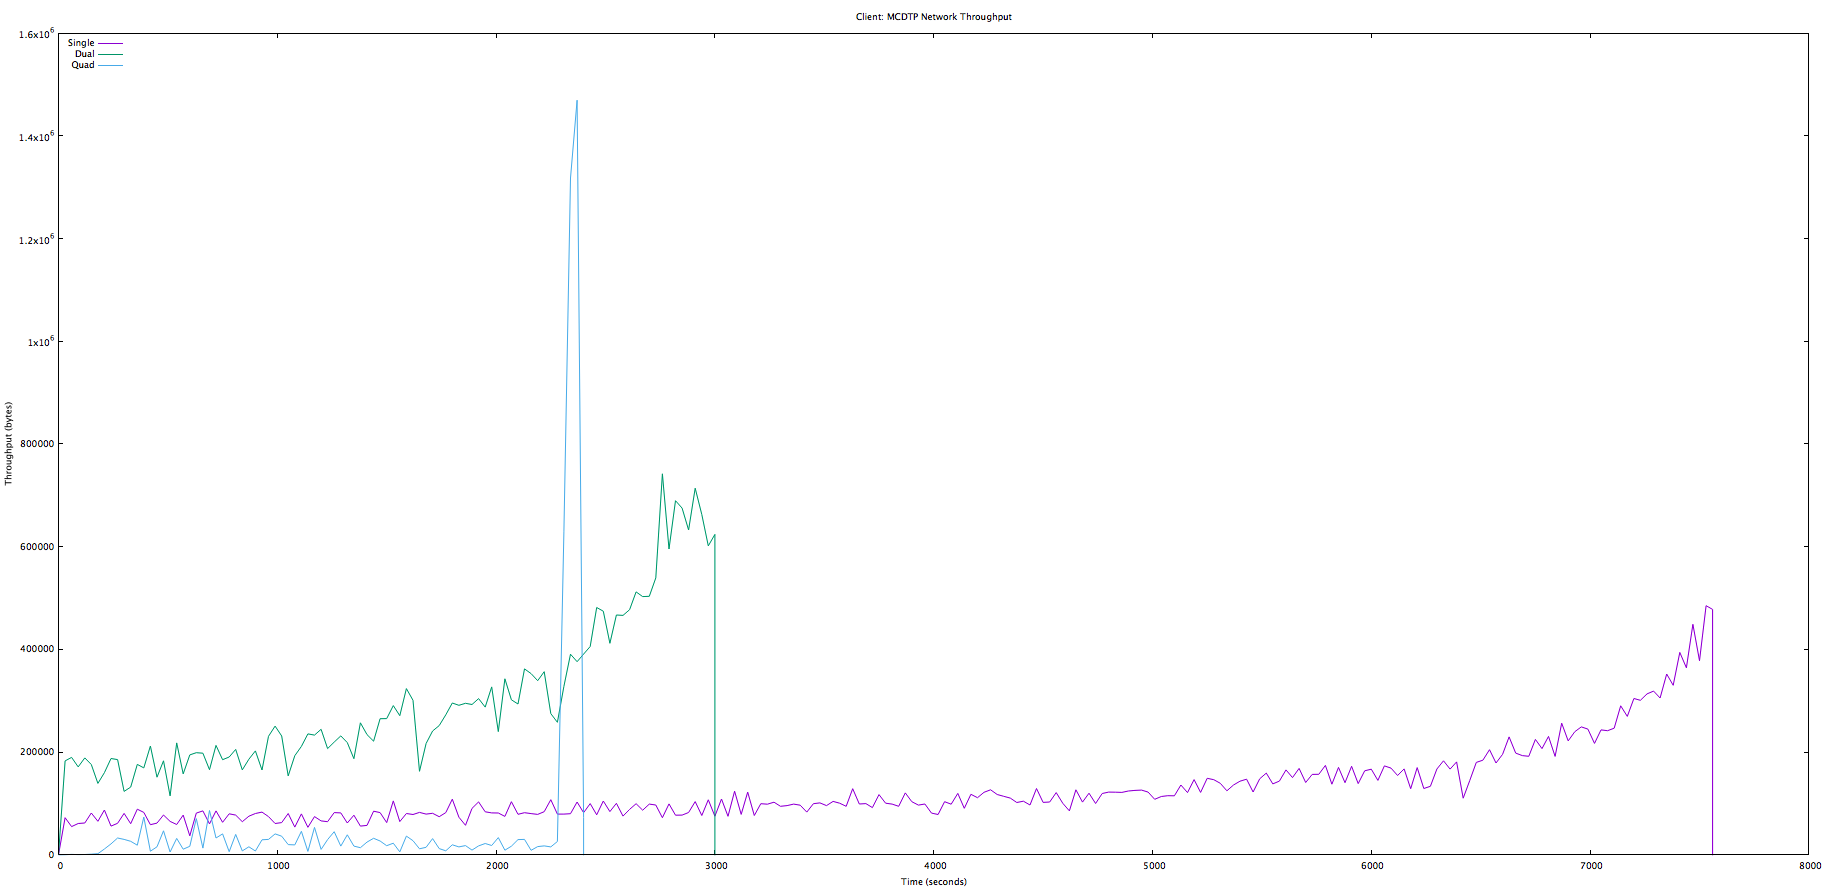
\includegraphics[scale=0.4]{TestResultClientThroughput}
\caption{Client Throughput}
\label{fig:tr-ct}
\end{figure}

\begin{figure}[ht]
\centering
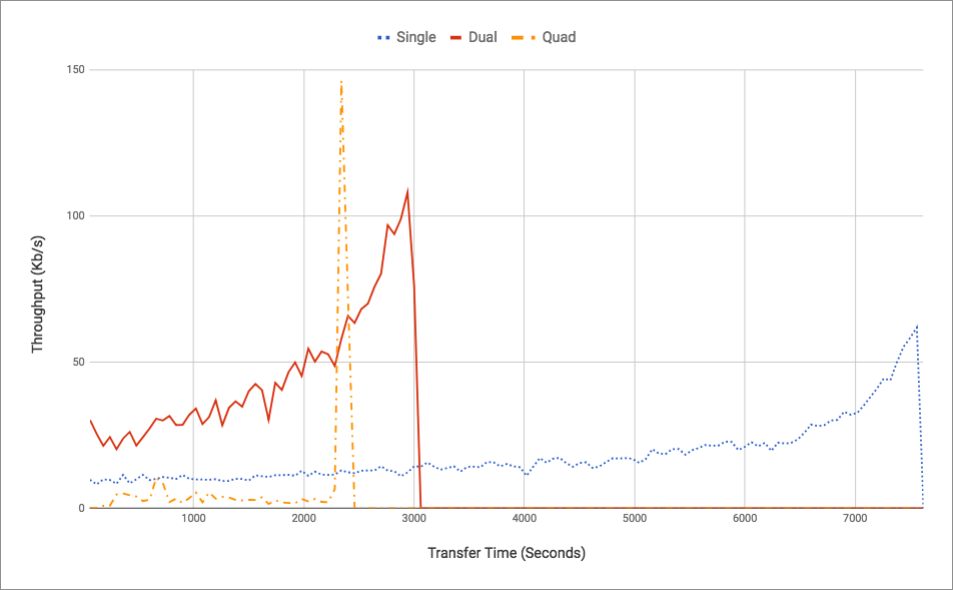
\includegraphics[scale=0.4]{TestResultServerThroughput}
\caption{Server Throughput}
\label{fig:tr-st}
\end{figure}

\begin{figure}[ht]
\centering
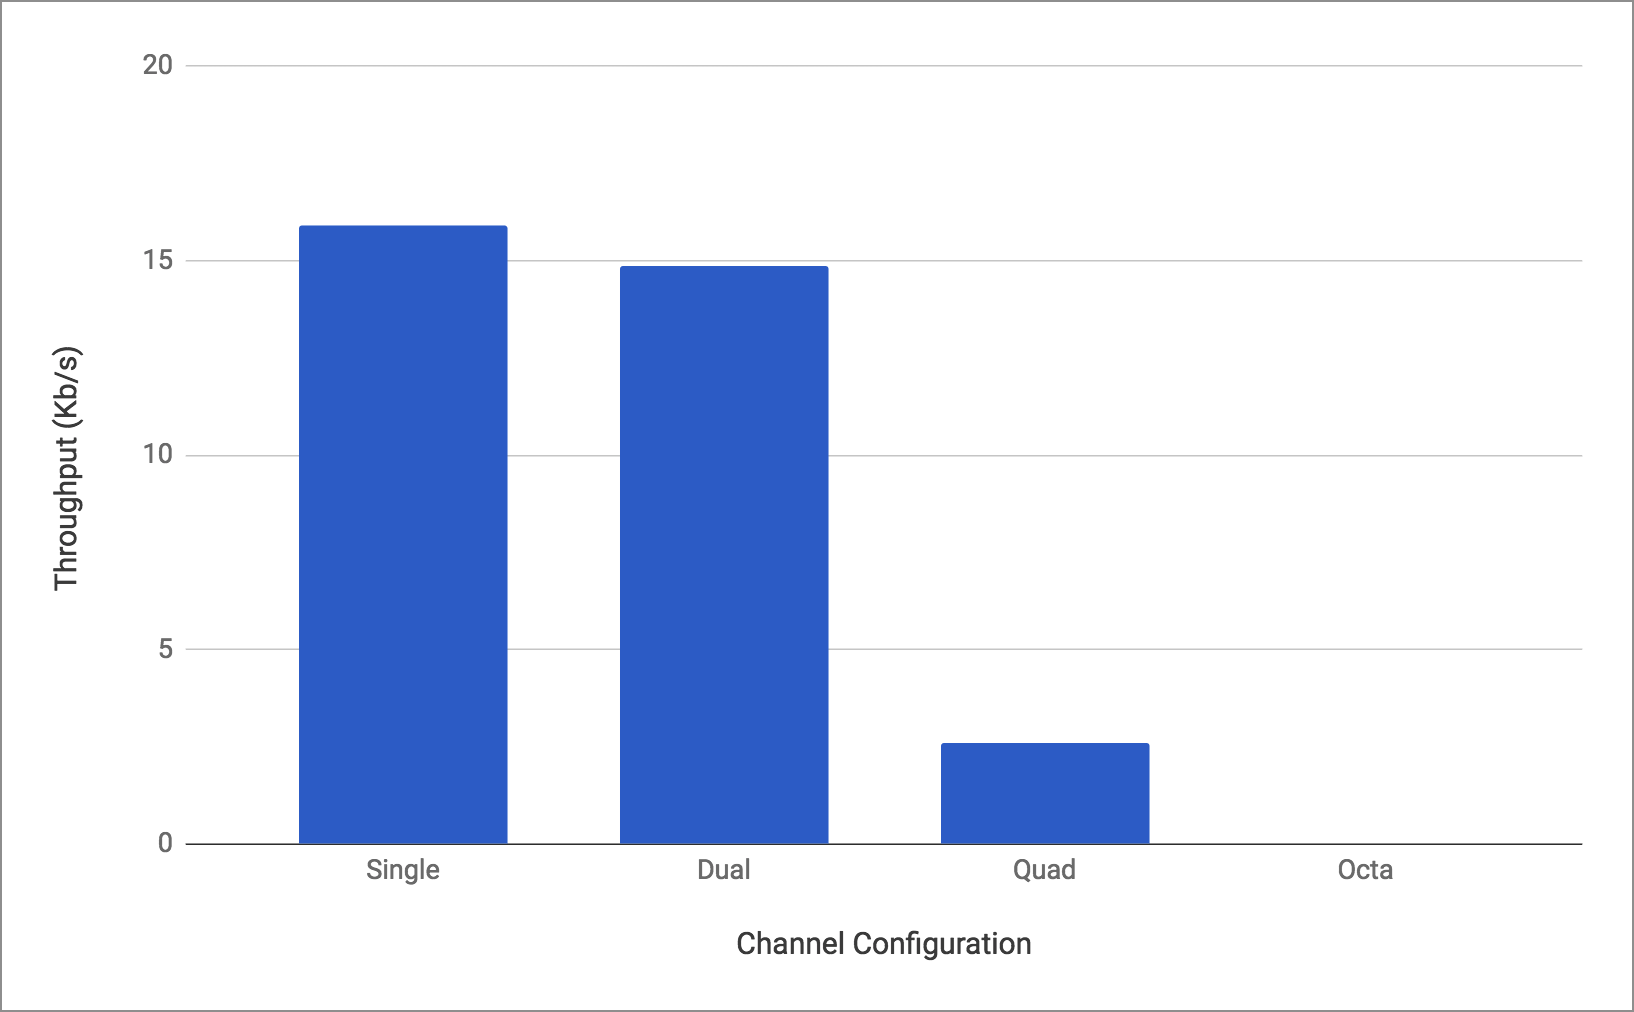
\includegraphics[scale=0.4]{TestResultAverageThroughput}
\caption{Average Throughput}
\label{fig:tr-at}
\end{figure}

\begin{figure}[ht]
\centering
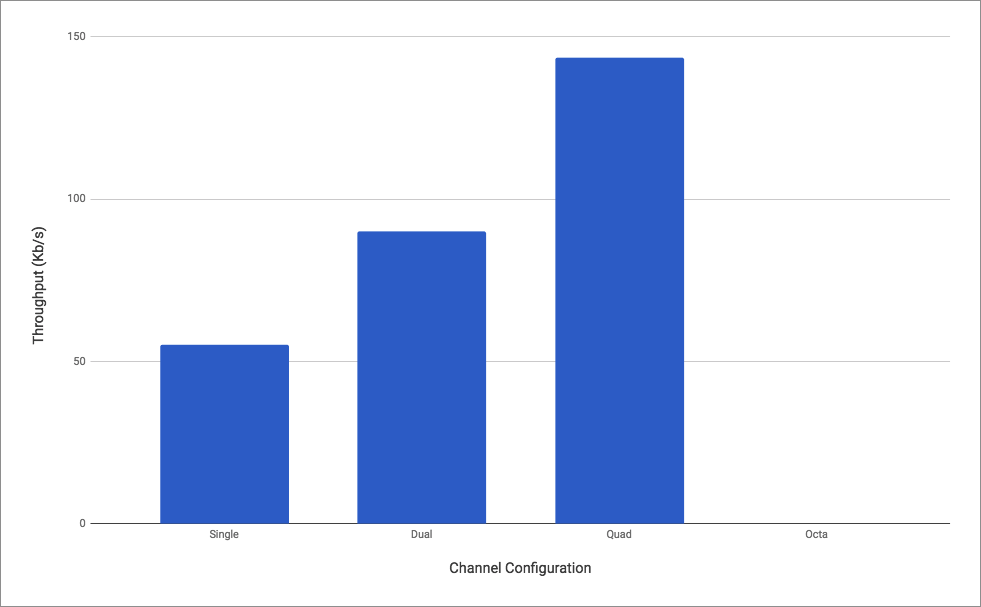
\includegraphics[scale=0.4]{TestResultMaxThroughput}
\caption{Max Throughput}
\label{fig:tr-mt}
\end{figure}

\begin{figure}[ht]
\centering
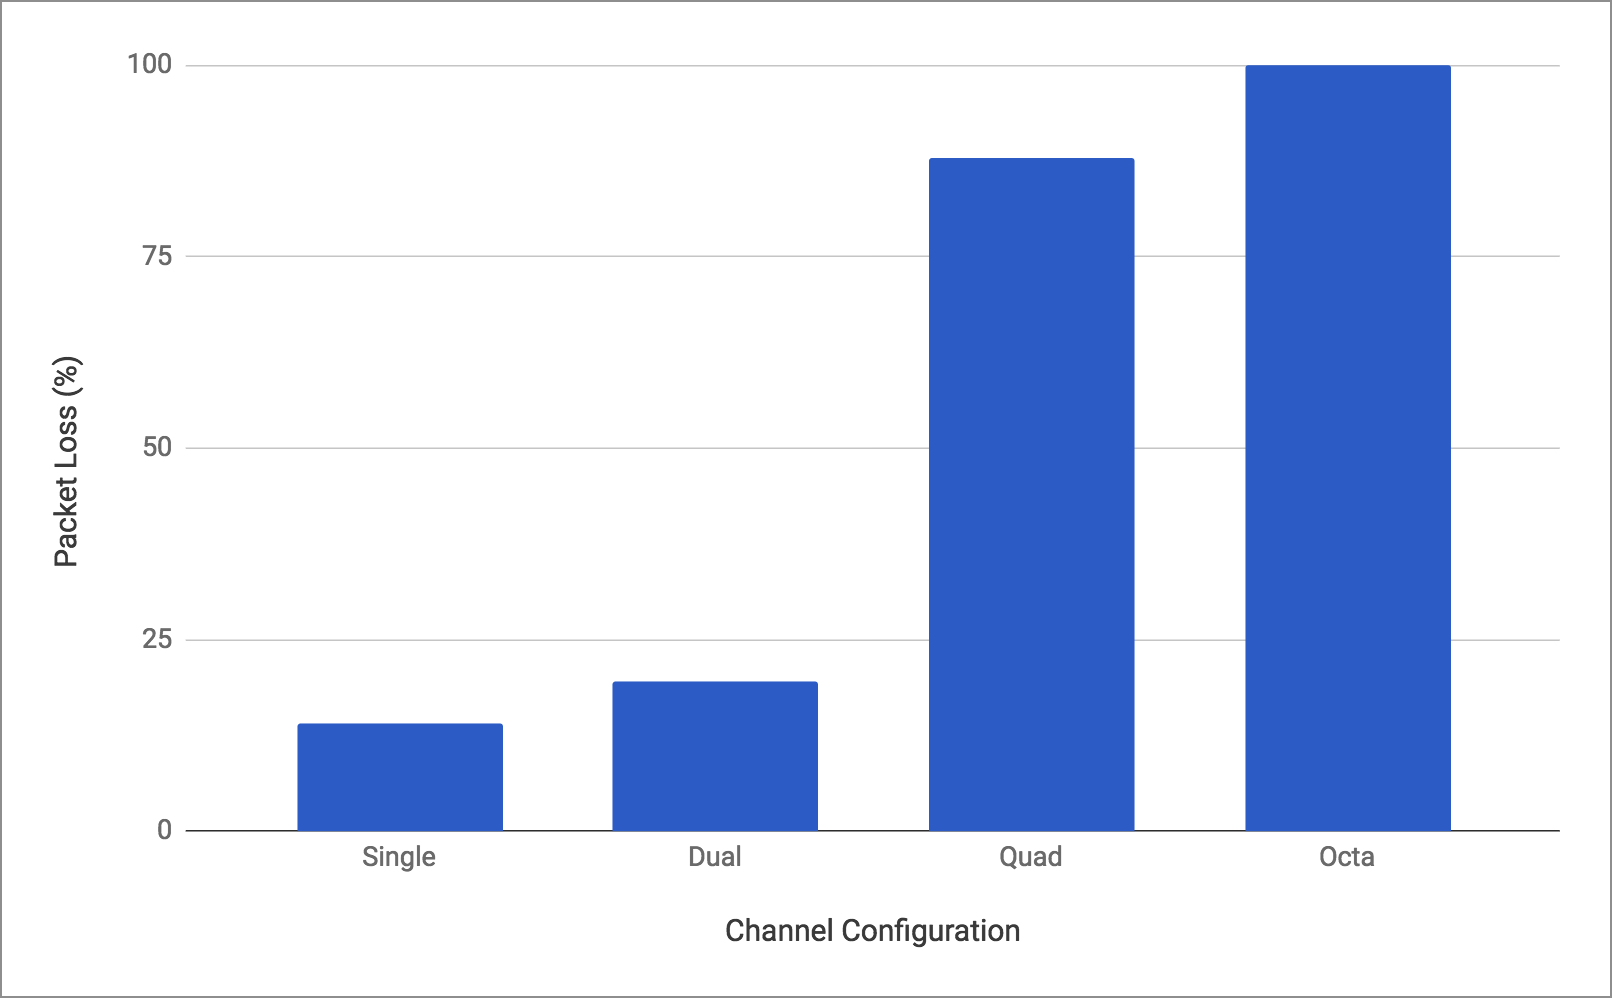
\includegraphics[scale=0.4]{TestResultPacketLoss}
\caption{Packet Loss}
\label{fig:tr-pl}
\end{figure} % Testing, Evaluation and Discussion

\chapter{Challenges and Future Work}\label{chp:c-fw}

\section{Challenges}

There were a number of challenges faced with this project. Some challenges derived from the language, others from poor design choices in early versions of MCDTP and MCDTPi. Challenges related to the language stemmed more from the .NET Framework. The discovered asynchrony issue in the cross-platform variant of the .NET Framework was rather obscure. With little documentation on the matter, a significant portion of the investigation involved examining the source code of both the .NET Core Framework and the Common Language Runtime. This was the only way to confirm that I/O Completion Ports were only being used on the Win32 Kernel API.

With respect to MCDTP and MCDTPi design challenges, early iterations had challenges with respect to disk I/O operations blocking socket I/O operations. The early architecture was not modular like MCDTPi is now. Consequently, MCDTPi needed to be restructured to be modular as discussed in Section \ref{sec:mod-arch} and incorporate asynchrony at an architectural level, which is discussed in Section \ref{sec:async-arch}. Additionally, MCDTP was originally designed to use file checksumming to determine which portions of the file needed retransmission. However, this proved to be very inconsistent, partly due to the slowness, and was replaced with the $PacketManagement$ system discussed in Section \ref{sec:pm-sm}.

\section{Future Work}

As mentioned in Chapter \ref{subsec:ftp-hs}, file selection was not included in the design of MCDTP. This feature was left out because it was outside the scope of the project and was left as future work for MCDTP and MCDTPi.

Tests have revealed that the .NET Core Framework does not use I/O Completion Ports on Unix-based operating systems. Testing IOCP is beyond the scope of this project. In order to understand how IOCP will impact performance, a separate study may need to be conducted. Since MCDTP and its implementation are open source, they can be used as candidate software to test the Windows environment. This would provide a direct comparison to Unix-based operating systems.

Asynchronous tasking is an overhead that could be mitigated. Restructuring MCDTPi to more efficiently use asynchrony would reduce the performance impact of TPL. Asynchronous tasks would need to be used on packets in bulk rather than per packet. This is only applicable to MCDTPi. The .NET Core Framework handles sending packets asynchronously and thus is infeasible to modify. Another option would be to implement a custom asynchronous module that tries to mitigate the effects of using TPL. These options would need to be explored in a separate study.

The data transmission phase could be optimized as well. As outlined in the design of MCDTP, a UDP packet can range from $13B \rightarrow 64KB$ in size. However, MCDTPi, is currently limited to $1500B$ in size due to the MTU of the network. Packets larger in size are fragmented to fit this within this limit. This limitation effects bandwidth usage. A path worth exploring to circymvent this would be to prefragment a $64KB$ chunk of data, it would likely need to be less than $64KB$ to account for any headers added to fragments, so that when fragmentation occurred, it would not fragment the data being transferred.
 % Challenges and Future Work

\chapter{Conclusion}

The design of MCDTP attempts to minimize overhead by keeping control messages minimalistic and employing a phase system for structured data transfers over each channel. Asynchrony was a major component to MCDTPi both architecturally and in implementation. In efforts to provide a continuous chain of asynchronous work flows from disk I/O to socket I/O, and vice versa, MCDTPi librally utilized the asynchronous technology built into the F\# language. This, coupled with the incomplete cross-platform support of the .NET Core Framework, produced behavior contrary to what was expected. As shown in this paper, using asynchrony excessively can have negative effects on performance in Computer Networking. While asynchrony has many benefits, in the context of Computer Networking, it should be used methodically. % Conclusion

%% ----------------------------------------------------------------
% Now begin the Appendices, including them as separate files

% \addtocontents{toc}{\vspace{2em}} % Add a gap in the Contents, for aesthetics

% \appendix % Cue to tell LaTeX that the following 'chapters' are Appendices

% \chapter{An Appendix}

Lorem ipsum dolor sit amet, consectetur adipiscing elit.	% Appendix Title

% \input{Appendices/AppendixB} % Appendix Title

% \input{Appendices/AppendixC} % Appendix Title

\addtocontents{toc}{\vspace{2em}}  % Add a gap in the Contents, for aesthetics
\backmatter

%% ----------------------------------------------------------------
\label{Bibliography}
\lhead{\emph{Bibliography}}  % Change the left side page header to "Bibliography"
\bibliographystyle{unsrt}
\bibliography{Bibliography}  % The references (bibliography) information are stored in the file named "Bibliography.bib"

\end{document}  % The End
%% ----------------------------------------------------------------